\renewcommand*\thechapter{}
\renewcommand*\thesection{\Alph{section}}
\chapter*{Appendix}
\chaptermark{Appendix}
\stepcounter{chapter}
\ifoot{Appendix}
\addcontentsline{toc}{chapter}{Appendix}

\section{Schematic of the Riemann Pump circuit for simulation}
\label{app:schematic}
\newpage
\begin{figure}[H]
	\centering
  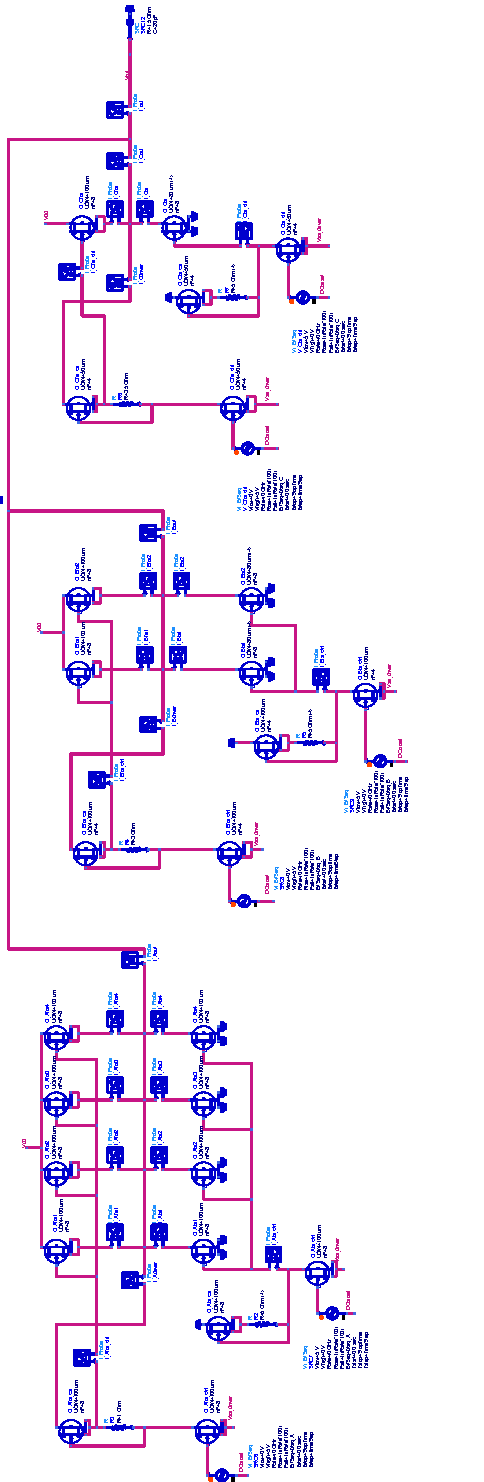
\includegraphics[scale = 1.35]{CircuitSchematic_portrait.pdf}
	\caption{Circuit for simulation}
	\label{fig:Circuitschematic}
\end{figure}

\section{Schematic of the realized Riemann Pump circuit}
\label{app:schematicRealizedPump}
\begin{figure}[H]
	\centering
  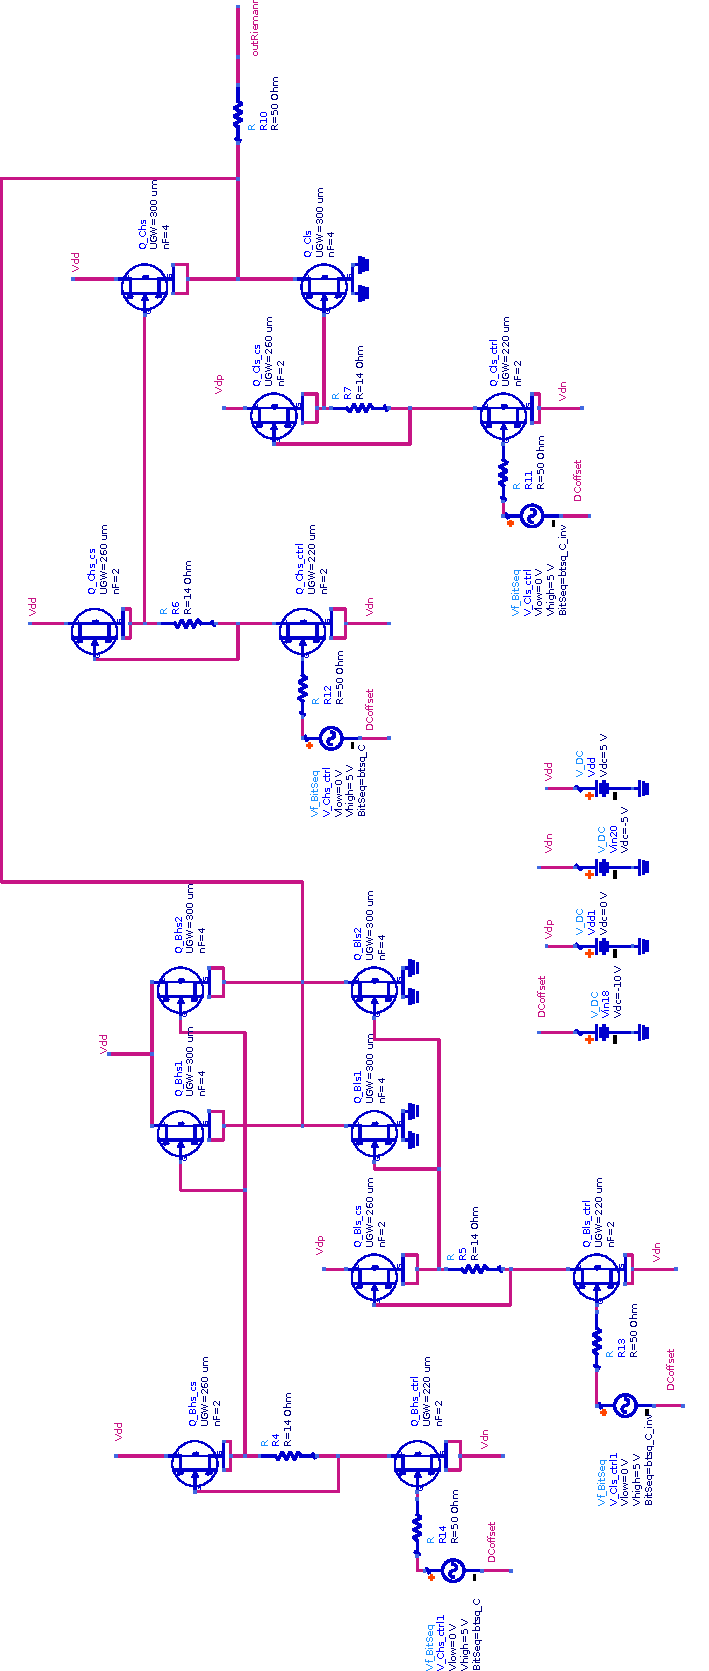
\includegraphics[scale=0.75]{realizedCircuit_full_DDRi_XY6.pdf}
	\caption{Realized test circuit with \gls{ab:ads}}
	\label{fig:RealCircuitschematic}
\end{figure}


\newpage
\section{Photography of the realized Demonstrator}

\begin{figure}[H]
   \centering
   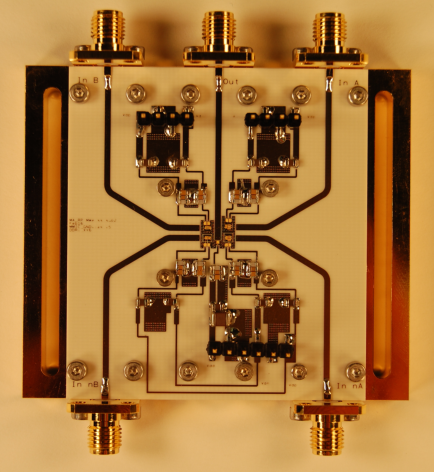
\includegraphics[width=\textwidth]{Demonstrator.pdf}
   \caption{Photo demonstrator}
   \label{pic:DemonstratorDDRiXY6}
\end{figure}

\newpage
\section{SNR Calculation for simulated signals}
\label{app:snr}
The calculation of the signal to noise ratio with the corresponding plots is stated here, for the generation of a sine wave with the Riemann Code:
\begin{equation}
000\hspace{.3cm} 010\hspace{.3cm} 101\hspace{.3cm} 111\hspace{.3cm} 111\hspace{.3cm} 101\hspace{.3cm} 010\hspace{.3cm} 000.
\end{equation}
Table \ref{tab:snr} states the parameter used for the desired theoretical sine wave.


\begin{table}[h]
\centering
\caption{Calculated SNR and corresponding parameters for the theoretical sine wave}
\label{tab:snr}
\begin{tabular}{|l|l|l|l|l|l|l|l|}
\hline
freqeuncy {[}GHz{]}   & 0.5           & 1           & 2             & 3             & 4             & 5             & 6             \\ \hline
\textbf{SNR {[}dB{]}} & \textbf{12.7} & \textbf{15} & \textbf{21.1} & \textbf{28.3} & \textbf{27.9} & \textbf{31.9} & \textbf{32.5} \\ \hline
amplitude {[}V{]}     & 7.5           & 7.5         & 6.5           & 4.5           & 3             & 2             & 1.75          \\ \hline
offset {[}V{]}        & 7.5           & 7.5         & 7.5           & 10            & 11.5          & 12.5          & 13            \\ \hline
phase {[}rad{]}       & pi/4          & pi/4        & 0             & -pi/16        & -pi/16        & -pi/8         & -pi/8         \\ \hline
\end{tabular}
\end{table}


\begin{figure}[h]
   \centering
   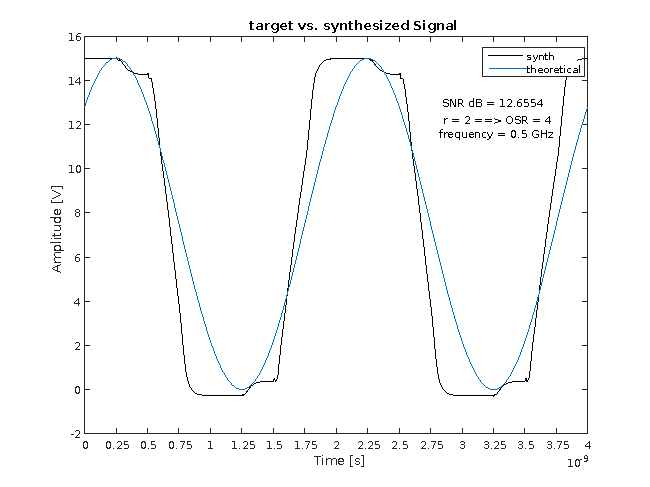
\includegraphics[width=0.9\textwidth]{FullSine05GHz.pdf}
   \caption{calculated SNR[dB]=12.7 sine wave (f = 0.5 GHz)}
   \label{fig:snr05GHz}
\end{figure}

\begin{figure}[h]
   \centering
   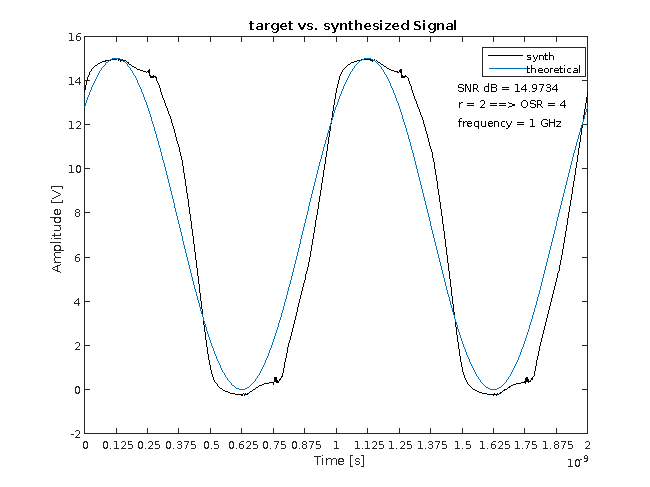
\includegraphics[width=0.9\textwidth]{FullSine1GHz.pdf}
   \caption{calculated SNR[dB]=15 sine wave (f = 1 GHz)}
   \label{fig:snr1GHz}
\end{figure}

\begin{figure}[h]
   \centering
   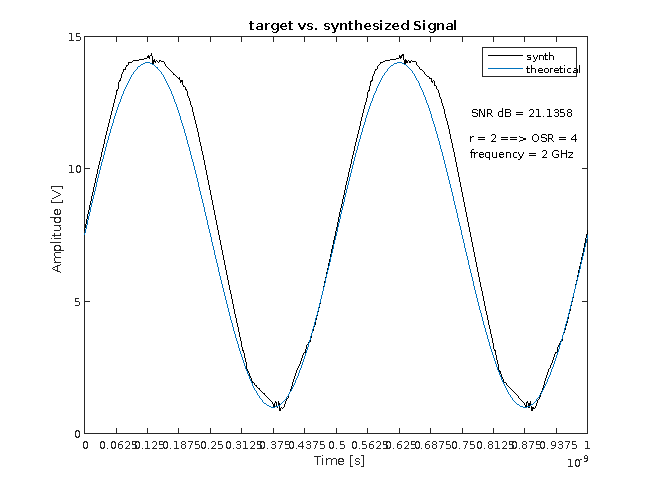
\includegraphics[width=0.9\textwidth]{FullSine2GHz.pdf}
   \caption{calculated SNR[dB]=21.1 sine wave (f = 2 GHz)}
   \label{fig:snr2GHz}
\end{figure}

\begin{figure}[h]
   \centering
   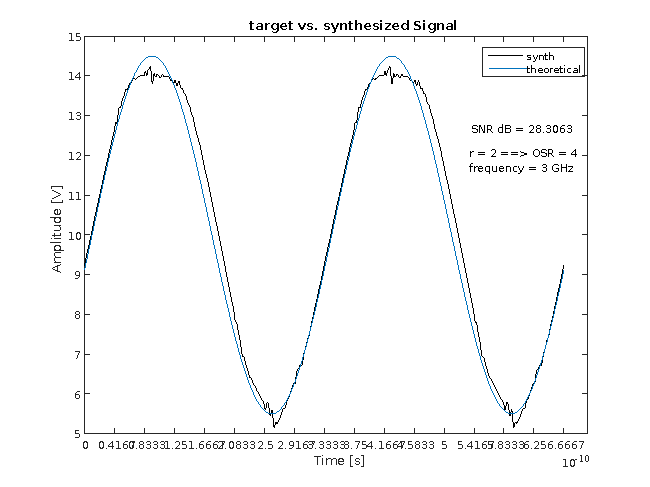
\includegraphics[width=0.9\textwidth]{FullSine3GHz.pdf}
   \caption{calculated SNR[dB]=28.3 sine wave (f = 3 GHz)}
   \label{fig:snr3GHz}
\end{figure}

\begin{figure}[h]
   \centering
   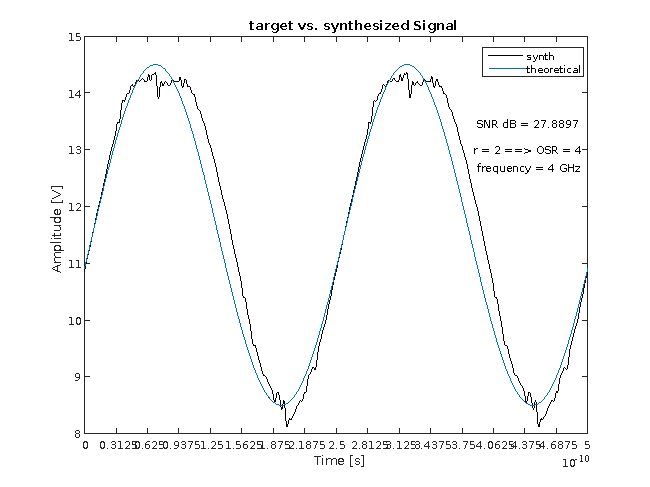
\includegraphics[width=0.9\textwidth]{FullSine4GHz.pdf}
   \caption{calculated SNR[dB]=27.9 sine wave (f = 4 GHz)}
   \label{fig:snr4GHz}
\end{figure}

\begin{figure}[h]
   \centering
   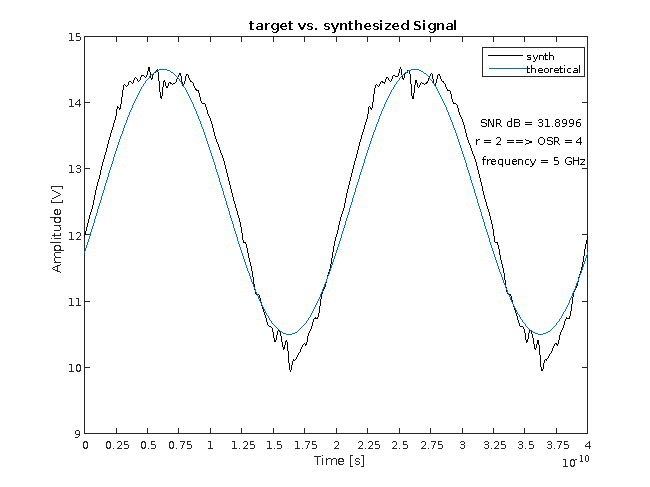
\includegraphics[width=0.9\textwidth]{FullSine5GHz.pdf}
   \caption{calculated SNR[dB]=31.9 sine wave (f = 5 GHz)}
   \label{fig:snr5GHz}
\end{figure}

\begin{figure}[h]
   \centering
   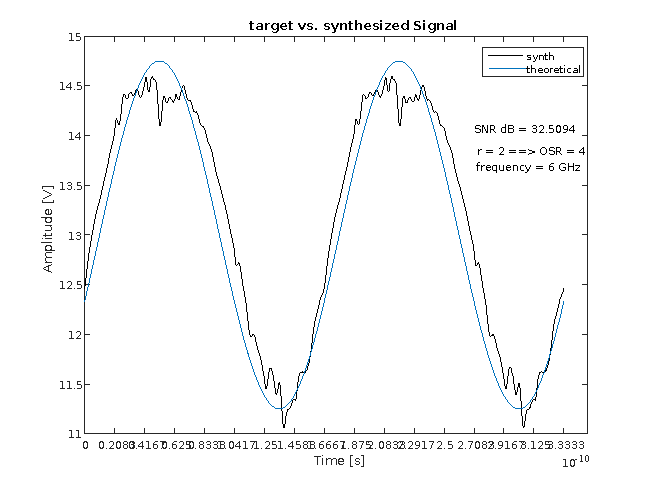
\includegraphics[width=0.9\textwidth]{FullSine6GHz.pdf}
   \caption{calculated SNR[dB]=32.5 sine wave (f=6 GHz)}
   \label{pic:DemonstratorDDRiXY6}
\end{figure}
